% MBA Speedrun -- OML group project report
% Overleaf: upload this folder (main.tex, refs.bib, figures/) and compile with pdfLaTeX + BibTeX.
\documentclass[11pt,a4paper]{article}

% ---------------------------------------------------------------- edit these
\newcommand{\groupmembers}{%
  Prathik          & PGPGC202500155 \\
  Nikita Naik Mood & PGPGC202500453 \\
  Anureet Biswas   & PGPGC202500109 \\
  Mrinal Bhaskar   & PGPGC202500338 \\}
\newcommand{\repourl}{\url{https://github.com/p25prathik-hue/mba-speedrun}}
\newcommand{\siteurl}{\url{https://p25prathik-hue.github.io/mba-speedrun/}}
% ----------------------------------------------------------------------------

\usepackage[a4paper,margin=2.5cm,headheight=14pt]{geometry}
\usepackage[T1]{fontenc}
\usepackage{lmodern}
\usepackage{microtype}
\usepackage{amsmath,amssymb}
\usepackage{graphicx}
\usepackage{booktabs,tabularx,longtable,array}
\usepackage[table]{xcolor}
\usepackage{float}
\usepackage[font=small,labelfont=bf]{caption}
\usepackage{enumitem}
\usepackage[most]{tcolorbox}
\usepackage[round,authoryear]{natbib}
\usepackage{fancyhdr}
\usepackage[hidelinks]{hyperref}
\usepackage{siunitx}
\setlist{itemsep=2pt,topsep=4pt}
\setlength{\parskip}{4pt}
\renewcommand{\arraystretch}{1.15}

\pagestyle{fancy}\fancyhf{}
\fancyhead[L]{\small MBA Speedrun}\fancyhead[R]{\small OML Group Project, IIM Ahmedabad}
\fancyfoot[C]{\small \thepage}
\renewcommand{\headrulewidth}{0.4pt}

\newtcolorbox{statusbox}[1][Status]{enhanced,colback=white,colframe=black,boxrule=0.9pt,arc=0mm,
  borderline={0.4pt}{2pt}{black},left=2mm,right=2mm,fonttitle=\bfseries\small,title={#1},fontupper=\small}
\newcommand{\est}{\textsuperscript{\textsc{est}}}

\begin{document}
% ============================================================== COVER
\begin{titlepage}
\centering
\vspace*{1.2cm}
{\large Optimisation Methods in Logistics (OML)\par}
{\large Indian Institute of Management Ahmedabad\par}
\vspace{2.2cm}
{\Huge\bfseries MBA Speedrun\par}
\vspace{0.4cm}
{\LARGE Personalised Learning Roadmaps\\[2pt] as a Sequential Ordering Problem\par}
\vspace{1.0cm}
{\large Sequencing PGP core micro-topics as a precedence-constrained asymmetric TSP,\\ split into daily study plans by bin packing\par}
\vspace{2.4cm}
{\large Group project report\par}
\vspace{0.8cm}
{\large
\renewcommand{\arraystretch}{1.25}
\begin{tabular}{ll}
\textbf{Group members} & \textbf{Roll No.} \\[2pt]
\groupmembers
\end{tabular}\par}
\vfill
{\large November 2026\par}
\vspace{0.3cm}
{\small Code and data: \repourl\par}
{\small Student roadmap planner: \siteurl\par}
\end{titlepage}

% ============================================================== ABSTRACT
\begin{abstract}
\noindent Almost every IIMA student faces a catch-up crunch before end-terms or summer-placement preparation. The PGP core is taught as parallel courses to a cohort of about 400, but a student catching up alone learns one topic at a time. We model the catch-up as a \emph{Sequential Ordering Problem} (SOP): an asymmetric TSP with precedence constraints in which the student is the machine, micro-topics are jobs, and the cost of moving from topic $i$ to topic $j$ is a sequence-dependent setup time, a classic TSP application. The formulation uses load variables $Q_i$ as ``study hours still to go'', which removes subtours and turns forgetting into a linear, capped cost. The data is a web of 266 micro-topics across all 37 first-year courses with 387 prerequisite links, checked against seven textbooks and three MIT syllabi: 88\% of the links that could be checked agree with their order. On this web the ordering heuristics (nearest neighbour, cheapest and farthest insertion, Clarke--Wright savings, or-opt and 2-opt) cut a fresh learner's estimated total from 502 hours, studying subject by subject, to 415 hours (17\%). Savings comes out as the best starting heuristic. Personalisation saves a further 28--79 hours, and keeping the 77 concepts shared by several courses in one web avoids about 142 hours of re-learning. Exact branch and bound, checked on a 28-topic Finance and Accounting pilot, proves optimality up to about 20 topics. On every pilot instance it could prove, the heuristics found the optimum. All times and cost parameters are estimates, and the gains survive $\pm25\%$ changes to every one of them. The model, data and a browser-based roadmap planner are on GitHub for future groups.
\end{abstract}

\tableofcontents
\newpage

% ============================================================== 1
\section{The IIMA problem}
\label{sec:problem}
Every PGP1 student has a version of the same week: an end-term in four days with half of Corporate Finance still unclear, or summer interviews in three weeks and a shaky grip on accounting. The core is designed for a cohort. About 400 students take parallel courses (FRA, Statistics, Economics, Marketing, Operations, and so on), sequenced around rooms, faculty and the trimester calendar. A student who is catching up alone faces a different problem: one learner, one topic at a time, and a fixed number of hours.

\paragraph{Decision.} Given a scope (topics to learn, topics already known, topics to skip) and $H$ study hours per day, find the order of micro-topics that
(i) respects every prerequisite, including prerequisites that cross courses;
(ii) minimises total time, counting the warm-up when switching subjects, the time saved when related topics are adjacent, and the revision needed when a prerequisite was learnt long ago; and
(iii) splits the order into days.

\paragraph{Why order matters at all.} If each topic took a fixed time regardless of what came before, every valid order would take the same total and any topological sort would do. Order matters because costs are \emph{sequence-dependent}. WACC is faster right after CAPM. Jumping from FRA to Marketing costs a warm-up. Using a prerequisite learnt 40 hours ago needs revision. These are exactly the ``distances'' $c_{ij}$ of a travelling salesman problem.

\paragraph{The logistics analogy.} The student is a single machine, topics are jobs with processing times $t_i$, $c_{ij}$ is a sequence-dependent setup time, prerequisites are precedence constraints, and days are bins of size $H$. The baseline is the curriculum order. We expect, honestly, that the curriculum is close to optimal for a student who learns everything in it. The gains should come from personalisation (skipping what you know), merged concepts, cross-course sequencing and avoiding forgetting.

\paragraph{No overlap with other groups.} Other groups model campus food delivery, water-can CVRP, elective bidding and placement panels. Ours is a learning-sequencing problem.

% ============================================================== 2
\section{Why it is hard, and the trade-offs}
\label{sec:hard}
\begin{enumerate}[leftmargin=*]
\item \textbf{NP-hard.} The SOP contains the asymmetric TSP, which is NP-hard. Even a 28-topic pilot has astronomically many orders, and the 266-topic IIMA web is far beyond enumeration.
\item \textbf{Precedence across courses.} 23\% of the 387 links cross domains (Figure~\ref{fig:domains}). Five cross-course prerequisites are taught \emph{later} in the timetable than the topic that needs them; for example, EVA in CCS (T2) needs WACC from Corporate Finance (T3).
\item \textbf{AND/OR prerequisites.} Some topics need one of several routes (3 OR groups in the web). In the pilot, incremental project cash flows can be reached through the cash-flow statement \emph{or} through relevant costing. This makes the closure itself an optimisation.
\item \textbf{Time-dependent costs.} Forgetting depends on how long ago a prerequisite was learnt, not only on its neighbour. So the cost is not a pure function of adjacent pairs, and the plain TSP cost matrix is not enough.
\item \textbf{Asymmetric, non-metric, partly negative costs.} $c_{ij}\neq c_{ji}$, and synergy makes some $c_{ij}<0$. The classical worst-case guarantees (nearest insertion $\le 2$, Christofides $\le 3/2$) need symmetric metric costs, so they do not apply. We measure empirical gaps instead.
\item \textbf{Estimated data.} Topic hours and cost parameters cannot be observed directly. Results must survive changes in them (Section~\ref{sec:sens}).
\end{enumerate}

\paragraph{Trade-offs.}
\textbf{Clustering vs integration}: finishing one subject first saves switching but leaves cross-course prerequisites idle until forgotten.
\textbf{Interleaving vs switching cost}: mixing subjects helps long-term retention in learning research \citep{rohrer2007}, but each switch costs a warm-up.
\textbf{Coverage vs time budget}: in a crunch you cannot do everything, so you choose by value per hour.
\textbf{Exactness vs scale}: branch and bound proves optimality up to about 20 topics; beyond that we rely on heuristics.

% ============================================================== 3
\section{Model and formulation}
\label{sec:model}
\paragraph{Sets and data.} $N=\{1,\dots,n\}$ topics in the student's scope (after closure, Sec.~\ref{sec:data}); dummy start $S$ and end $E$. $p_i=m_it_i$ is the effective time, where $m_i<1$ for partial prior knowledge. $T=\sum_i p_i$. $A$ is the set of AND links $k\to j$; $G_j$ the OR groups of $j$; $\mathcal{S}$ the SOFT links. All parameters below are estimates\est{} in hours.

\paragraph{Transition cost.} For $j$ studied immediately after $i$,
\[
c_{ij} \;=\; w\,[\mathrm{dom}_i\neq\mathrm{dom}_j] \;-\; s\,\mathrm{sim}(i,j)\,p_j ,
\]
where $w=0.5$ is the warm-up for a subject switch and $s=0.15$ is the share of $p_j$ saved right after a fully related topic. $\mathrm{sim}=1$ along a prerequisite link, $0.5$ against it or for adjacent sessions of a course, $0.25$ for the same course, and otherwise an explicit overlap value. A first-topic warm-up $c_{Sj}=0.5$ is constant.

\paragraph{Variables.} $x_{ij}\in\{0,1\}$: $j$ follows $i$. $Q_i\in[p_i,T]$: study hours still to go just before starting $i$. $y_{kj}\in\{0,1\}$: OR member $k$ is the one used by $j$. $v_{kj}\in\{0,1\}$: SOFT link violated. $r_{kj}\ge 0$: revision hours. $b_{kj}\in\{0,1\}$: the refresh cap is active.

\begin{align}
\min\;& \textstyle\sum_i p_i + \sum_{(i,j)} c_{ij}x_{ij} + \sum r_{kj} + \pi\sum v_{kj} \label{eq:obj}\\
\text{s.t. }& \textstyle\sum_j x_{ij}=1 \;\; \forall i\in N\cup\{S\} \qquad \sum_i x_{ij}=1 \;\; \forall j\in N\cup\{E\} && \text{(I), (II)}\label{eq:deg}\\
& Q_i \ge Q_j + p_i x_{ij} - T(1-x_{ij}),\quad Q_i \le Q_j + p_i + T(1-x_{ij}) && \text{load}\label{eq:load}\\
& Q_k \ge Q_j + p_k \quad \forall (k\to j)\in A && \text{AND}\label{eq:and}\\
& \textstyle\sum_{k\in G} y_{kj}\ge 1,\quad Q_k \ge Q_j + p_k - T(1-y_{kj}) && \text{OR}\label{eq:or}\\
& Q_k \ge Q_j + p_k - T v_{kj} \quad \forall (k\to j)\in\mathcal S && \text{SOFT}\label{eq:soft}\\
& r_{kj} \ge \rho\,(Q_k - p_k - Q_j - L) - \rho T b_{kj},\quad r_{kj} \ge \kappa p_k\, b_{kj} && \text{forgetting (capped)}\label{eq:rev}
\end{align}
with $Q_S=T$, $Q_E=0$. The first inequality in \eqref{eq:load} is the load-based subtour-elimination constraint used in compact vehicle-routing models, with each topic's hours as its ``load''; it removes subtours. The second makes $Q$ an exact clock, so $Q_k-p_k-Q_j$ is exactly the number of study hours between finishing $k$ and starting $j$. Together, the two inequalities in \eqref{eq:rev} give $r_{kj}=\min\{\rho(\text{gap}-L)^+,\ \kappa p_k\}$. Revision starts after $L=12$ hours at rate $\rho=0.02$ hours per hour of gap, and a refresh never costs more than $\kappa=0.5$ of the prerequisite's own time. The binary $b_{kj}$ is needed only for links whose gap could reach the cap. In an OR group revision applies only to the member used. A SOFT violation costs $\pi=1$ hour.

\paragraph{A lesson from scaling up.} The first version had no cap: forgetting grew linearly without limit. On the 28-topic pilot this was harmless, because no gap is long. On the 266-topic web a T1 prerequisite used in T3, about 300 study hours later, was charged about 6 hours of revision on \emph{every} link, and the timetable order came to 956 hours for 382 hours of study. The cap ($\kappa$) is the realistic fix: a forgotten topic needs a refresh, not a second course. It changes no pilot result, and it is one of the parameters tested in Section~\ref{sec:sens}.

\paragraph{Valid inequalities.} If $k$ is an AND-ancestor of $j$, then $x_{jk}=0$; $x_{Sj}=0$ if $j$ has a prerequisite in scope; $x_{iE}=0$ if $i$ has a dependent in scope; $x_{ij}+x_{ji}\le 1$ (subtour breaking for $|S|=2$); and $p_i+\sum_{\text{desc}}p \le Q_i \le T-\sum_{\text{anc}}p$.

\paragraph{Second stage: days.} For the chosen order, a day covering topics $a{+}1..b$ takes $h_{ab}=\omega+\sum p+\sum c$ hours, where $\omega=0.25$ is the day warm-up. The split minimises days, then hours, subject to $h_{ab}\le H$ (Sec.~\ref{sec:days}).

\paragraph{Crunch variant.} Add $z_i\in\{0,1\}$ for ``topic $i$ studied'', replace the right-hand sides of (I) and (II) by $z_i$, enforce precedence only when $z_j=1$ (with $z_j\le z_k$ for every AND link), and solve $\max\sum r_iz_i$ subject to total hours $\le C$.

The model objective was checked against an independent evaluator of any sequence: they agree to machine precision on every instance tested, and on small instances the MILP optimum equals brute-force enumeration (\texttt{tests/test\_core.py}).

% ============================================================== 5
\section{Data and the topic web}
\label{sec:data}
\begin{statusbox}[Two datasets]
\textbf{The IIMA web} (266 micro-topics, 37 courses, 387 links after Step~1) is the main dataset: every profile, crunch and sensitivity result in Sections~\ref{sec:results} and~\ref{sec:sens} uses it. \textbf{The pilot} (28 Finance and Accounting topics built from textbook contents pages) is small enough for exact branch and bound. It is used only to measure how good the heuristics and bounds are. Topic hours, values and cost parameters are \textbf{estimates} in both; only the course list is official.
\end{statusbox}

\paragraph{The 266-topic IIMA web.} Micro-topics cover all 37 official first-year courses (Table~\ref{tab:domains}). Each topic has a primary course, every other course that also teaches it, a first term, a size (45, 90 or 150 minutes) and a value from 1 to 5. Links are AND (required), OR (one of a group) or SOFT (helpful). The starter-kit audit, re-run with path-fixed scripts that reproduce the original files byte for byte, gives the following:
\begin{itemize}
\item 383 links: 364 AND, 6 OR in 3 groups, 13 SOFT;
\item no cycles, and 9 redundant links removed by transitive reduction;
\item 77 topics taught in more than one course (merged concepts, 169 course tags);
\item 23\% of links cross domains; one isolated topic (ENV05);
\item longest chain 16 topics; 381.8 hours of base study time.
\end{itemize}
Our own checks (Kahn's sort and the Bellman--Ford negative-cycle test) agree on every count. Figure~\ref{fig:domains} shows where the required links cross domains: Quant feeds Finance, Operations and Economics, and Accounting feeds Finance.

\begin{table}[H]\centering\small
\caption{The 266-topic web by domain. Hours are estimates.}\label{tab:domains}
\begin{tabular}{@{}lrr@{\hspace{2em}}lrr@{}}
\toprule
Domain & Topics & Hours & Domain & Topics & Hours\\
\midrule
Quant \& Analytics & 43 & 61.8 & OB \& HR & 20 & 26.2\\
Finance & 35 & 56.5 & Strategy & 16 & 22.8\\
Accounting & 34 & 50.2 & Research Methods & 10 & 14.2\\
Economics & 29 & 45.0 & IT \& Digital & 8 & 10.5\\
Operations & 27 & 36.5 & Ethics, Society \& Env & 7 & 9.8\\
Marketing & 25 & 34.0 & Law & 7 & 7.5\\
 & & & Communication & 5 & 6.8\\
\midrule
\multicolumn{3}{@{}l}{\textbf{Total}: 266 topics, 381.8 hours} & & & \\
\bottomrule
\end{tabular}
\end{table}

\paragraph{Five curriculum timing gaps.} The audit compares each link with the terms in which the two topics are first taught. Five links point backwards in time (Table~\ref{tab:gaps}). A student who follows the timetable meets the dependent topic before its prerequisite.

\begin{table}[H]\centering\small
\caption{Prerequisites taught after the topic that needs them.}\label{tab:gaps}
\setlength{\tabcolsep}{4pt}\begin{tabular}{@{}p{4.1cm}lp{4.6cm}ll@{}}
\toprule
Prerequisite & Course (term) & Needed by & Course (term) & Link\\
\midrule
WACC & CF (T3) & Performance measures: ROI, RI, EVA & CCS (T2) & AND\\
Goal of the firm and agency problems & CF (T3) & Corporate governance & LAB (T1) & AND\\
Questionnaire and survey design & BRM (T3) & Conjoint analysis & MKT-II (T2) & AND\\
Value chain analysis & SM (T3) & Digital transformation and IT strategy & TBIT (T2) & SOFT\\
Goal of the firm and agency problems & CF (T3) & Stakeholder theory and CSR & PCE (T2) & SOFT\\
\bottomrule
\end{tabular}
\end{table}

\begin{figure}[H]\centering
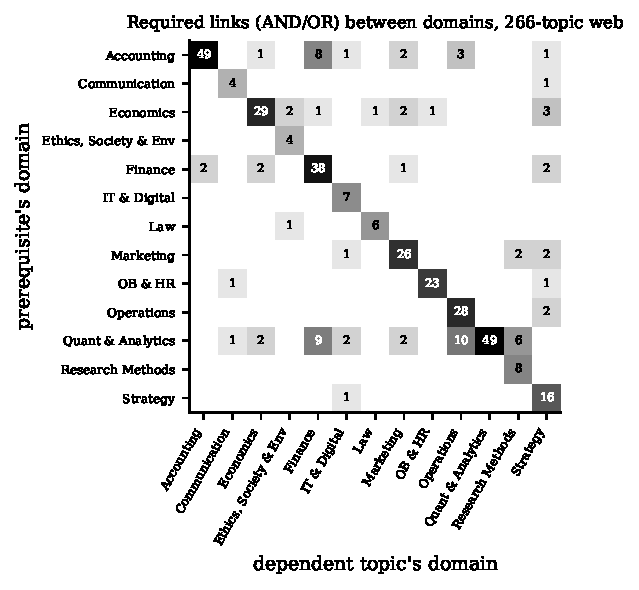
\includegraphics[width=0.62\linewidth]{figures/fig_domains.pdf}
\caption{Required (AND/OR) links between domains in the 266-topic web. The diagonal holds within-domain chains; off-diagonal cells are the cross-course prerequisites that make sequencing a single problem rather than 13 separate ones.}
\label{fig:domains}
\end{figure}

\paragraph{The pilot.} 28 micro-topics in four domains: financial reporting (8), statistics (2), management accounting (7) and corporate finance (11). They take 71.5 hours\est{} and are joined by 38 links (26 AND, 10 SOFT, one OR group); the full list is in Appendix~\ref{app:topics} and the web is drawn in Figure~\ref{fig:web}. It was built independently of the IIMA web, from textbook and syllabus order.

\begin{figure}[H]\centering
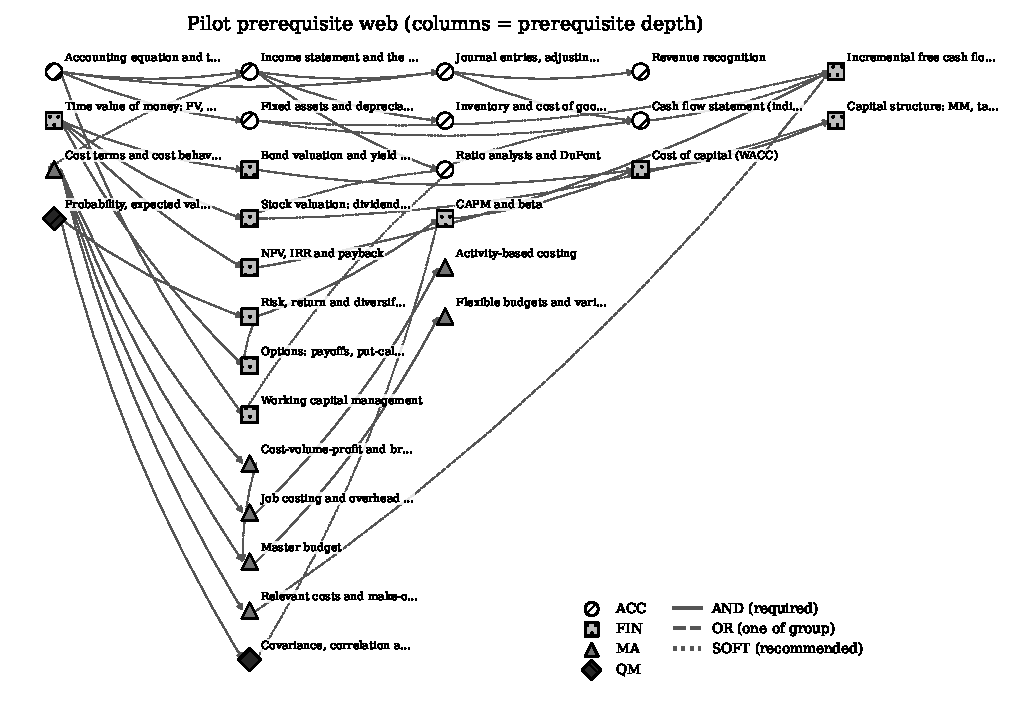
\includegraphics[width=\linewidth]{figures/fig_web.pdf}
\caption{The pilot prerequisite web, used for the exact-method checks. Columns show prerequisite depth.}
\label{fig:web}
\end{figure}

\subsection{Step 1: external sources for the links}
We searched for credible evidence on how MBA topics relate.
\begin{itemize}
\item \textbf{Concept-prerequisite datasets.} LectureBank covers NLP, ML, AI, deep learning and IR (later also computer vision and bioinformatics) \citep{li2019lecturebank}. MOOCCube and MOOCCubeX annotate prerequisites for psychology, mathematics and computer science on Chinese MOOCs \citep{yu2020mooccube,yu2021mooccubex}. Neither covers the MBA core, and we found no public dataset that does. That gap is part of the case for this project's web.
\item \textbf{Accreditation.} AACSB's 2020 standards set competency goals but are not prescriptive about courses or their order \citep{aacsb2020}. We use them for framing only.
\item \textbf{Textbooks and syllabi (used).} We used the chapter order of seven core texts:
\begin{itemize}
\item Brealey--Myers--Allen--Edmans \citep{bma2023};
\item Horngren's \emph{Cost Accounting} \citep{datar2021};
\item Cachon--Terwiesch \citep{cachon2024};
\item Anderson et al.'s business statistics \citep{asw2020};
\item Kotler--Keller \citep{kotler2024};
\item Pindyck--Rubinfeld \citep{pindyck2021};
\item Robbins--Judge \citep{robbins2019};
\end{itemize}
plus Mankiw's \emph{Macroeconomics} \citep{mankiw2022} and the session order of MIT OCW 15.401, 15.511 and 15.501 \citep{ocw15401,ocw15511,ocw15501}.
\end{itemize}
We record only order facts and paraphrased unit names, never textbook text, and only chapters whose order we could confirm.

\paragraph{Method.} 129 of the 266 topics were mapped by hand to chapters or sessions (147 mappings; \texttt{data/iima/topic\_unit\_map.csv}). A link $u\to v$ \emph{agrees} with a source when both topics map to that source and $u$'s unit comes earlier, and \emph{disagrees} when it comes later. Order is weak evidence, because a later chapter need not depend on an earlier one, so agreement only upgrades a link's \texttt{source} label; it never creates a link by itself.

\paragraph{Result.} 119 of the 383 links fall within at least one source. Of the 95 judgements that compare different chapters, 84 agree and 11 disagree, an agreement rate of \textbf{88\%}. A further 40 judgements fall within the same chapter. We reviewed every disagreement:
\begin{itemize}
\item \textbf{Six AND links downgraded to SOFT}, because the textbook teaches the ``dependent'' first:
  \begin{itemize}
  \item graphical before numerical descriptive statistics;
  \item payout policy before MM;
  \item network effects with demand, long before monopoly;
  \item oligopoly before game theory;
  \item personal selling before channel design;
  \item emotions before personality.
  \end{itemize}
\item \textbf{Five kept, with a note.} Futures before options has mixed evidence: MIT agrees with our link, Brealey--Myers does not. One mismatch comes from mapping a broad topic to one chapter. Three involve the go-to-market plan, which our web treats as a capstone while Kotler--Keller introduces planning first.
\end{itemize}
We also \textbf{added four SOFT links} where a source shows a real build-up:
\begin{itemize}
\item bonds before stock valuation;
\item option pricing before real options;
\item balance sheet before income statement;
\item the newsvendor model before safety stock.
\end{itemize}
The web now has 387 links (358 AND, 6 OR, 23 SOFT). It is still acyclic, every ID is unchanged, and \texttt{prereqs.csv} has a \texttt{source} column: 119 links carry a textbook or syllabus label, and 268 remain our estimates. Every decision and its reason is in \texttt{data/external/step1\_changes\_iima.csv}. On the pilot the same procedure gives 90\% agreement, but that figure is circular, because the pilot was built from the same sources.

% ============================================================== 6
\section{Solution methods}
\label{sec:methods}
\paragraph{Personalisation and closure.} A profile lists known topics (treated as done), skipped topics, partial knowledge ($m_i$), target topics or domains, and an optional crunch budget. If a required prerequisite is outside the scope, it is added back with a warning. For an OR group, the member with the cheapest closure is added.

\paragraph{Baselines.} \textbf{B0, timetable order}: terms in sequence, with parallel courses interleaved within a term as a student attending classes meets them, then repaired by Kahn's algorithm (a dependent waits for a prerequisite taught later). \textbf{B1, subject by subject}: finish one course, then the next. This is cluster-first, route-second, the logic of the sweep heuristic.

\paragraph{Construction.} A topic is \emph{available} once its AND prerequisites and at least one member of each OR group are done.
\begin{itemize}
\item \emph{Nearest neighbour} appends the available topic with the smallest true increment: $c_{ij}$ plus the revision it triggers at the current clock.
\item \emph{Cheapest insertion} inserts an available topic $k$ at the position minimising $\Delta_{ijk}=c_{ik}+c_{kj}-c_{ij}$ after its prerequisites.
\item \emph{Farthest insertion} places the hardest topic first.
\item \emph{Savings} starts with one chain per topic and merges the chain ending in $i$ with the chain starting at $j$ in decreasing $s_{ij}=c_{i0}+c_{0j}-c_{ij}$, skipping a merge if it would create a cycle among chains. That is the same question Kruskal's algorithm asks, here on directed chains, and includes the case where another chain would have to sit between the two.
\end{itemize}

\paragraph{Improvement.} \emph{Or-opt} moves blocks of $p=3,2,1$ topics to their best position inside the window between the block's last prerequisite and first dependent. \emph{2-opt} reverses a segment only if it contains no internal prerequisite, and re-costs it, because $c_{ij}\ne c_{ji}$. The two alternate until neither improves. Every construction and baseline is improved this way, and random feasible orders give restarts.

\paragraph{Exact method.}
\label{sec:exact}
CBC branch and bound \citep{pulp} on \eqref{eq:obj}--\eqref{eq:rev} with the valid inequalities, warm-started with the heuristic tour. Lower bounds: the assignment relaxation with arc fixing, and the LP relaxation with and without cuts.

\paragraph{Days.}
\label{sec:days}
Sorting topics by size, as first-fit decreasing does, would break prerequisites, so the order stays fixed. The \emph{exact} split is a shortest path: nodes are positions $0..n$, and an arc $a\to b$ is ``one day covering topics $a{+}1..b$''. It is allowed if $h_{ab}\le H$, and its cost is lexicographic (one day, then $h_{ab}$ hours). It has the same structure as the classic shortest-path model for production lot sizing. A switch placed at a day break costs nothing extra, because every day starts with a warm-up anyway. ``Can I finish in $D$ days?'' is answered by a hop-limited Bellman--Ford search. Every plan is reported next to the bin-packing bound $\lceil\sum p_i/H\rceil$.

\paragraph{Crunch.} The \emph{profit-maximising tour heuristic} grows the plan by the topic, together with its missing prerequisites, that gives the most value per hour actually consumed after cheapest insertion. The usual bang-for-buck ratio $(r_i-\delta_i)/d_i$ assumes value and cost in the same money units; here value and hours are different units, so the ratio is value $\div$ hours added. Several initial tours are tried and the best is kept. Two exact references check it: the prize-collecting MILP, and the capital-budgeting knapsack with $z_j\le z_k$, which ignores sequencing effects. Topics left out are the ``common carrier'' list: candidates for a senior's session or peer notes.

\paragraph{Implementation.} The model is in Python (\texttt{src/speedrun}). Evaluating one order of 266 topics takes about 7\,$\mu$s with an optional compiled evaluator (Numba) that performs exactly the same arithmetic; without Numba a vectorised NumPy evaluator takes about 30\,$\mu$s and agrees to within $10^{-12}$\,h. One full local search then takes 1--3\,s. There are 19 tests:
\begin{itemize}
\item brute force on small instances, including cases where the revision cap binds;
\item split optimality, closure and the null model;
\item JavaScript parity on both webs;
\item the NumPy evaluator against the plain loops, and the plain-language front end.
\end{itemize}
The website runs a line-by-line JavaScript port of the heuristics, which reproduces the Python results exactly for every preset. For scopes of more than 120 topics the browser uses only the two strongest constructions, so that it answers in a few seconds.

% ============================================================== 7
\section{Results across profiles}
\label{sec:results}
\subsection{Five students on the 266-topic web}
Table~\ref{tab:profiles} compares four hour totals for each profile:
\begin{itemize}
\item replaying the whole first year in timetable order (the naive baseline);
\item the student's own scope in timetable order (B0, parallel courses interleaved);
\item the scope subject by subject (B1, one course after another in term order);
\item our roadmap.
\end{itemize}
Each total counts study, switching (net of synergy) and revision. The roadmap is the best of the NN, CI, FI and savings constructions and both baselines, each improved by or-opt and 2-opt, plus five random restarts.

\begin{table}[H]\centering\small
\caption{Results on the 266-topic web at $H=6$ h/day. Hours\est{} = study + switching + revision + SOFT penalties. Scope gain = naive baseline -- B0. Sequencing gain = B1 -- roadmap (B0 -- roadmap in brackets).}
\label{tab:profiles}
\setlength{\tabcolsep}{4pt}
\begin{tabular}{@{}lrrrrrrrr@{}}
\toprule
Profile & Topics & Study h & B0 & B1 & Roadmap & Scope gain & Seq.\ gain & Days (LB)\\
\midrule
Fresh learner & 266 & 381.8 & 673.9 & 502.3 & 415.4 & -- & 86.9 (258.5) & 72 (64)\\
Engineer & 257 & 357.8 & 622.9 & 451.3 & 385.8 & 51.0 & 65.5 (237.1) & 68 (60)\\
Commerce graduate & 252 & 344.8 & 594.8 & 443.3 & 367.4 & 79.1 & 75.9 (227.4) & 64 (58)\\
Skip Marketing & 255 & 368.3 & 646.2 & 484.2 & 401.5 & 27.6 & 82.7 (244.7) & 69 (62)\\
\bottomrule
\end{tabular}\par\smallskip
{\footnotesize Naive baseline = 673.9\,h for everyone. ``Summers in 3 weeks'' is the crunch profile; see below.}
\end{table}

\begin{figure}[H]\centering
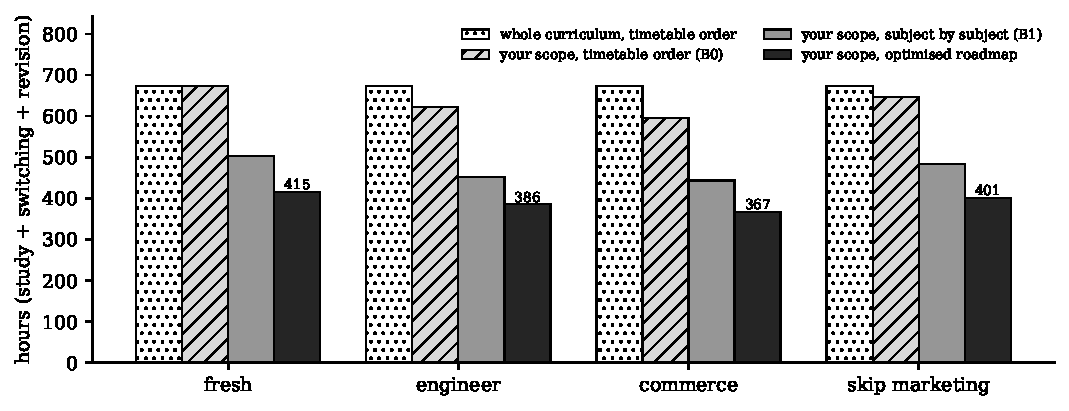
\includegraphics[width=\linewidth]{figures/fig_profiles.pdf}
\caption{Hours by profile on the 266-topic web.}
\label{fig:profiles}
\end{figure}

\begin{figure}[H]\centering
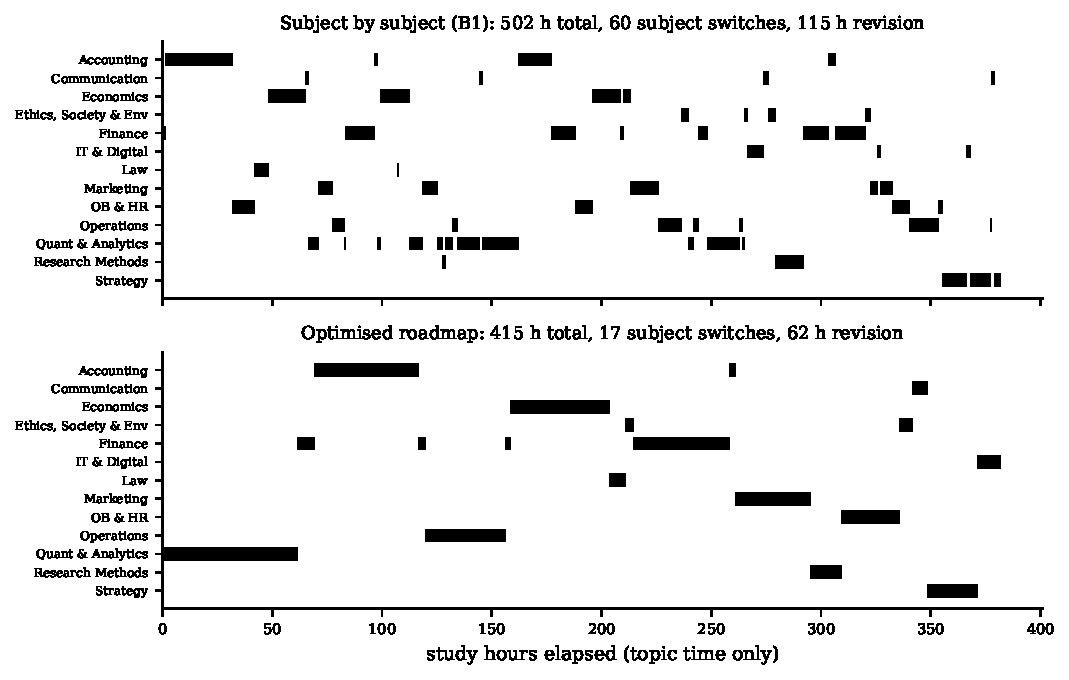
\includegraphics[width=\linewidth]{figures/fig_swimlanes.pdf}
\caption{When each domain is studied, for the fresh learner. Subject by subject (top) follows the timetable's course boundaries, so Accounting, Finance and Economics are each split across terms. The roadmap (bottom) learns each domain end to end across its courses, in the order the cross-domain prerequisites allow.}
\label{fig:swim}
\end{figure}

\paragraph{Reading the results.}
\begin{enumerate}[leftmargin=*]
\item \textbf{The roadmap saves 15--17\% against subject by subject} (65--87\,h). For the fresh learner, the 86.9\,h saving is made up of:
\begin{itemize}
\item less forgetting: revision falls from 115.1\,h to 62.2\,h;
\item better adjacency: net switching falls from $-2.6$\,h to $-28.6$\,h, with 17 subject switches instead of 60;
\item no violated SOFT links: 8.0\,h saved.
\end{itemize}
Against the timetable order the saving is 38\%, but that baseline switches subject 240 times and is not how anyone catches up alone.
\item \textbf{Learn a subject end to end, not term by term} (Figure~\ref{fig:swim}). The optimised order is \emph{more} clustered than subject by subject, but by domain rather than by course. FRA and CCS go together, then FM and CF together, ordered so that Quant comes first and Strategy last. Clustering by course splits a domain across terms and forces revision when it resumes.
\item \textbf{Personalisation saves 28--79\,h} (engineer 51\,h, commerce graduate 79\,h). This part does not depend on the estimated $c_{ij}$ at all.
\item \textbf{``Skipping Marketing'' skips less than half of it.} The closure adds back 14 of the 25 Marketing topics, because Strategy, BRM and Internet businesses need them: segmentation and positioning for innovation strategy, the marketing plan for the integrative case, and customer lifetime value for unit economics. Only 11 topics (13.5\,h of study) can really go, for a 27.6\,h total saving.
\item \textbf{Merged concepts are worth about 142\,h.} 77 topics are taught in several courses (169 course tags). Learning each one once in a shared web, instead of once per course, avoids about 142\,h of re-learning. This assumes a student would otherwise re-learn a concept in full in each course that teaches it, so it is an upper estimate.
\item \textbf{Clarke--Wright savings is the best start} for three of the four profiles, with farthest insertion best for the engineer. For the fresh learner, savings gives 430.4\,h before improvement and 415.4\,h after; nearest neighbour gives 474.1\,h and 428.1\,h.
\end{enumerate}

\paragraph{Crunch: summers in three weeks.} With a 60-hour budget (3\,h a day for 20 days) the profit-maximising tour picks 52 topics worth 218 of the 1{,}041 value points (21\%) in 59.95\,h:
\begin{itemize}
\item mostly Quant (14 topics), Accounting (12), Finance (10) and OB \& HR (10);
\item a few Strategy (4) and Operations (2) topics.
\end{itemize}
The sequence-blind knapsack reaches 216 points for the same hours. Everything left out is the ``common carrier'' list for seniors' sessions and peer notes. The values are estimates of placement relevance; a group with interview data should replace them.

\subsection{Exactness vs scale on the pilot, and how good the heuristics are}
The 266-topic web is far beyond exact methods, so we measured the heuristics on the pilot. We drew 21 random precedence-closed sub-instances of 8--28 topics and solved each by the heuristics and by CBC with a 180\,s limit (Table~\ref{tab:scale}, Figure~\ref{fig:scale}).

\begin{table}[H]\centering\small
\caption{Pilot: branch and bound vs heuristics on random sub-instances. Bound gaps are $(z^*-\text{LB})/z^*$, where $z^*$ is the best known value. Times were measured on a shared 2-core machine.}
\label{tab:scale}
\setlength{\tabcolsep}{4.5pt}
\begin{tabular}{@{}rrrrrrrrr@{}}
\toprule
$n$ & Inst. & Proven & B\&B s (med.) & Max nodes & Heur.\ gap (h) & LP & Assign.+fix & LP+cuts\\
\midrule
8 & 4 & 4 & 0.02 & 0 & 0 & 4.6\% & 0.8\% & 0.4\%\\
12 & 4 & 4 & 0.07 & 2 & 0 & 4.2\% & 1.1\% & 0.8\%\\
16 & 4 & 4 & 1.55 & 1{,}146 & 0 & 5.0\% & 1.6\% & 1.5\%\\
20 & 4 & 4 & 2.70 & 3{,}122 & 0 & 4.7\% & 1.4\% & 1.2\%\\
24 & 4 & 2 & 152 & 39{,}548 & 0$^\dagger$ & 5.1\% & 2.4\% & 2.3\%\\
28 & 1 & 0 & 180 (limit) & 33{,}228 & 0.001$^\ddagger$ & 5.8\% & 3.6\% & 3.6\%\\
\bottomrule
\end{tabular}\par\smallskip
{\footnotesize $^\dagger$Equal to CBC's best solution, but optimality is not proven. $^\ddagger$CBC's 180\,s incumbent is 0.001\,h better than the heuristic's 3-restart result; with 12 starts the heuristic finds 67.83\,h, better than CBC's 67.844\,h (notebook 3).}
\end{table}

\begin{figure}[H]\centering
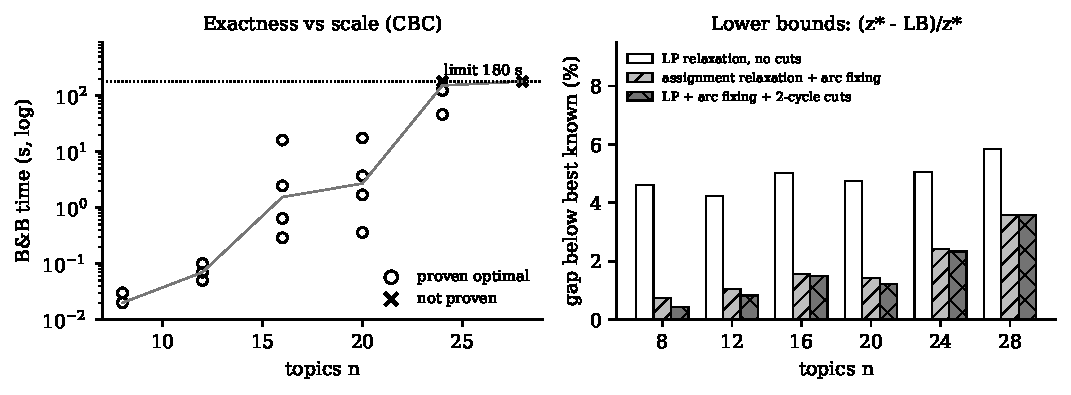
\includegraphics[width=\linewidth]{figures/fig_scale.pdf}
\caption{Pilot. Left: B\&B time grows roughly exponentially with $n$ (log scale). Right: lower bounds. Precedence arc fixing closes most of the LP gap; the assignment relaxation with the same fixing is almost as tight and far cheaper.}
\label{fig:scale}
\end{figure}

Three findings follow.
\begin{itemize}
\item \textbf{Exactness stops at about 20 topics} once forgetting costs are in the model. Every instance up to 20 topics was proven within 18\,s, 2 of 4 at 24 topics, and none at 28. The original plan had estimated 20--40 topics.
\item \textbf{The heuristics are reliable where we can check them.} On all 18 instances that B\&B proved optimal, the heuristic gap is zero. On the unproven instances the heuristic equals CBC's best solution, or is within 0.001\,h of it.
\item \textbf{Improvement does the work.} The best construction alone is up to 2.0\,h off at $n=20$ and 4.2\,h off at $n=28$; or-opt and 2-opt close that gap. On the 266-topic web, local search takes Clarke--Wright savings from 430.4\,h to 415.4\,h.
\end{itemize}

\paragraph{Crunch, exact vs heuristic (pilot).} At budgets of 15 and 25\,h the profit-maximising tour equals the exact prize-collecting MILP (23 and 39 value points). At 40\,h it finds 59 against the exact 60: one point (1.7\%) short.

\subsection{Days}
\begin{figure}[H]\centering
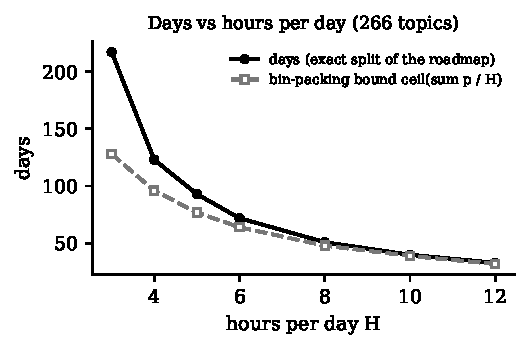
\includegraphics[width=0.55\linewidth]{figures/fig_days.pdf}
\caption{Days needed for the fresh learner's roadmap vs hours per day, against the bin-packing bound.}
\label{fig:days}
\end{figure}
At 6\,h/day the fresh learner's roadmap takes 72 days, against a bound of 64. Topics are indivisible, so small days waste capacity: at 3\,h/day the plan needs 217 days against a bound of 128, while at 10\,h/day it needs 40 days against 39. The exact shortest-path split never needs more days than greedy filling. Given the choice, it puts subject switches at day breaks, where the day's warm-up is paid anyway.

\section{Sensitivity analysis: are the results an artefact of estimated costs?}
\label{sec:sens}
Every hour and cost parameter is an estimate, so this is the weakest point of the model. We test it in three ways.

\paragraph{1. Null test.} With $w=s=\rho=\pi=0$, every feasible order costs exactly the study time (381.75\,h on the full web, 71.5\,h on the pilot), and the measured sequencing gain is exactly 0 on both webs. The code invents no gains.

\paragraph{2. One at a time, $\pm25\%$ (266-topic web, fresh learner).} Against subject by subject, the roadmap's gain stays between 15.6\% and 19.6\% for every parameter at $\pm25\%$; against the timetable order it stays between 35.5\% and 41.7\%. The most influential inputs are revision cap $\kappa$ (15.6--18.9\%), all topic hours (16.3--19.6\%) and the switch warm-up $w$ (16.1--18.1\%). The SOFT penalty barely matters. Following the nominal plan under a changed parameter costs between $-2.1$ and $3.1$ hours, under 1\% of the 415-hour total.

\paragraph{3. Monte Carlo.} Every topic's hours and every parameter were multiplied independently by $U[0.75,1.25]$, and each draw was re-optimised.
\begin{itemize}
\item \textbf{266-topic web, 60 draws.} The roadmap beat subject by subject in \textbf{all 60} draws, by a mean of 16.7\% (90\% of draws between 14.8\% and 18.6\%). It beat the timetable order by 37.6\% (34.8--40.1\%).
\item \textbf{Regret of the nominal plan} (what a student loses by following our plan when the true costs differ) averages $-0.8$\,h, between $-4.6$ and $4.8$\,h, and is positive in only 33\% of draws. At 266 topics, the heuristic's own run-to-run variation (about $\pm5$\,h, 1\%) is larger than the effect of $\pm25\%$ input errors on which plan is best. In practice the nominal plan is as good as re-optimising.
\item \textbf{Pilot, 200 draws} (with more restarts). The roadmap beat subject by subject in all draws, by 3.3\% (2.5--4.0\%), and the timetable order by 7.4\% (6.3--8.3\%). The nominal plan's regret was 0.12\,h. The pilot's gains are smaller because its chains are short and its gaps rarely trigger forgetting.
\end{itemize}

\begin{figure}[H]\centering
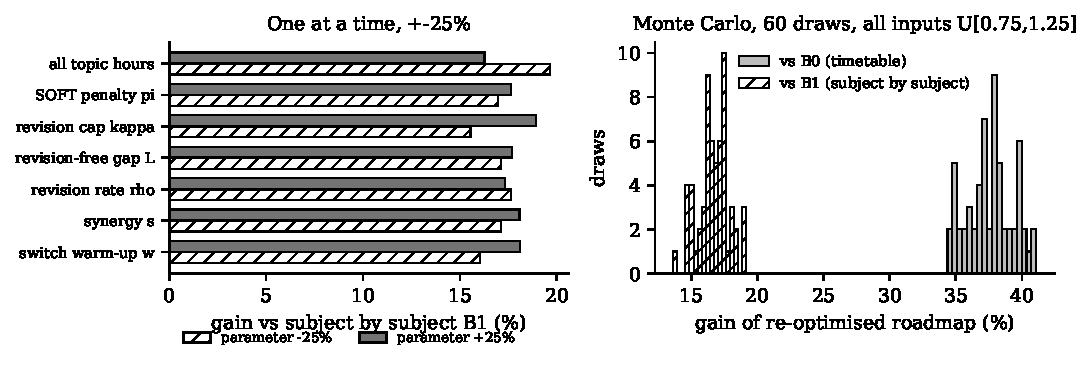
\includegraphics[width=\linewidth]{figures/fig_sensitivity.pdf}
\caption{266-topic web, fresh learner. Left: gain vs subject by subject (B1) with each parameter at $\pm25\%$. Right: Monte Carlo with all inputs at $\pm25\%$; neither distribution comes near zero.}
\label{fig:sens}
\end{figure}

\paragraph{What this does and does not show.} The \emph{size} of the sequencing gain depends on the estimates, most of all on the forgetting parameters. Its \emph{sign}, and the conclusion that a domain-clustered roadmap beats course-by-course study, hold throughout the $\pm25\%$ range. Following the nominal plan when the true costs differ costs little. Three things are \emph{not} tested:
\begin{itemize}
\item \textbf{A wrong functional form.} If interleaving improved long-term retention in a way our cost ignores \citep{rohrer2007,cepeda2006}, the true optimum would mix subjects more.
\item \textbf{Per-link forgetting.} Revision is charged per link, so a prerequisite used by many later topics may be counted more than once. This inflates revision for every order and favours orders that keep chains together.
\item \textbf{Scope gains are a separate matter.} They do not use $c_{ij}$ at all, so these tests neither strengthen nor weaken them.
\end{itemize}

\section{Insights}
\label{sec:insights}
\paragraph{For students.}
\begin{enumerate}[leftmargin=*]
\item \textbf{Cut scope first.} Prior knowledge saves 50--80 hours. Check what you cannot skip, though: ``skipping Marketing'' still leaves 14 of its 25 topics, because Strategy, BRM and Internet businesses build on them.
\item \textbf{Learn a domain end to end, not term by term.} Doing all of Accounting (FRA with CCS), then all of Finance (FM with CF), in prerequisite order saves about 17\% over going course by course. Most of the saving is forgetting avoided.
\item \textbf{Never replay the timetable when catching up alone.} Interleaving a dozen parallel courses suits a cohort and costs a solo learner the most: 240 subject switches and the most revision of any baseline.
\item \textbf{Shared concepts are one topic, not five.} WACC, regression and the cash-flow statement recur across courses. Learn each once, and you avoid about 142 hours of re-learning across the first year.
\item \textbf{Plan in blocks of about 6 hours or more if you can.} With 3-hour days, about 40\% of day capacity is lost to topics that do not fit.
\item \textbf{In a crunch, rank by value per hour, prerequisites included.} Hand the left-out list to a senior's session.
\end{enumerate}

\paragraph{For the curriculum and the Acads committee.}
\begin{enumerate}[leftmargin=*]
\item \textbf{Five timing gaps} (Table~\ref{tab:gaps}) send T1--T2 students to T3 material: WACC for EVA, agency theory for governance and CSR, survey design for conjoint, and the value chain for IT strategy. A one-session primer or pre-read in the earlier course would close each one.
\item \textbf{The cohort is limited by chains; a solo learner by total hours.} The longest chain in the web is 16 topics and about 26\,h of study, against 382\,h of content. Parallel courses are the right design for 400 students, and a roadmap tool for the solo learner complements them rather than replacing them.
\item \textbf{Shared concepts are a facility-location question.} Should a concept used by several courses be taught once (one ``facility'') or repeated? That is the UFLP trade-off between fixed cost and service distance, and a natural next project.
\item \textbf{A small data ask.} Publishing micro-topic hours in course outlines, or running a 10-minute PGP2 survey, would replace our estimates. The guidelines point to exactly this route (data from the Acads Secretary).
\end{enumerate}

\section{Limitations}
\label{sec:limits}
\begin{itemize}[leftmargin=*]
\item \textbf{Estimates.} Topic hours, values, the topic-to-course mapping and all six cost parameters are estimates. Only the course list is official.
\item \textbf{Cost form.} Switching, synergy and forgetting are linear (forgetting with a cap) and measured on a study-hour clock, not calendar time. Revision is charged per link, which can double-count a heavily used prerequisite. Interleaving benefits for retention are not modelled.
\item \textbf{Weak external evidence.} Chapter order is ordering evidence, not proof of dependence. 268 of the 387 links still rest on our judgement alone, and no public MBA prerequisite dataset exists to validate against.
\item \textbf{Heuristics at scale.} Optimality is proven only on pilot instances of up to about 20 topics. On the 266-topic web the reported roadmap is the best found, not a proven optimum.
\item \textbf{Indivisible topics, one learner.} A topic is never split across days. Group study (several machines) is not modelled.
\item \textbf{No field test.} A small trial with PGP1 volunteers before end-terms would be the real test.
\end{itemize}

\section{How to use and extend the GitHub tool}
\label{sec:github}
\paragraph{For students.} Open the website at \siteurl{} (the \texttt{docs/} folder of \repourl, published with GitHub Pages). It loads the 266-topic web by default. Go to the \emph{Roadmap planner}:
\begin{itemize}
\item tick what to skip;
\item mark topics as \emph{New}, \emph{Some} or \emph{Know it};
\item set hours per day, and choose \emph{Full roadmap} or \emph{Crunch}.
\end{itemize}
The heuristics run live in the browser, in a few seconds for the full web, and presets also show the Python result. The planner states in plain language any prerequisite it had to add back. Two explorers show what each topic needs and unlocks: ours, and the starter kit's detailed one (\texttt{docs/topic-web.html}, rebuilt by \texttt{scripts/kit/layout.py}).

\paragraph{Running the Python tool.} Students who want the Python version need not type commands. On Windows they download the repository and double-click \texttt{START\_HERE\_Windows.bat}; on a Mac or Linux they run \texttt{bash start\_mac\_linux.sh}. The first run installs what it needs. A menu then opens the planner, makes a roadmap or a crunch plan from a few plain questions (areas known, half known or skipped, and hours per day), and saves the plan as a CSV. The same questions are a form in a Google Colab notebook, opened from the README with one click.

\paragraph{For future groups.} Every module documents its method and assumptions in its docstring.
\begin{verbatim}
python -m pip install -r requirements.txt
python scripts/kit/audit.py      # rebuild from topics_source.txt
python scripts/integrate_external.py  --data data/iima
python scripts/apply_step1_changes.py --data data/iima
python run.py audit       --data data/iima
python run.py profiles    --data data/iima --out results/iima
python run.py sensitivity --data data/iima --draws 60
python run.py web         --data data/iima --out docs/data/web.json
python -m pytest -q
\end{verbatim}
Natural extensions: real hours from a survey; exam weights as values; group study as a VRP (several students = several vehicles); exam dates as time windows; and the UFLP for shared concepts. \texttt{CONTRIBUTING.md} lists the rules: keep IDs stable, label every estimate, and document the method used.

\bibliographystyle{plainnat}
\bibliography{refs}

% ============================================================== APPENDICES
\appendix
\section{Pilot topic list (the 266-topic web is in \texttt{data/iima/topics.csv})}
\label{app:topics}
{\small
\begin{longtable}{@{}lp{6.3cm}lrrp{3.3cm}@{}}
\toprule
ID & Topic & Domain & Term & Hours\est & Prerequisites (type)\\
\midrule\endhead
A1 & Accounting equation and the balance sheet & ACC & 1 & 3.0 & --\\
A2 & Income statement and the accrual principle & ACC & 1 & 2.5 & A1\\
A3 & Journal entries, adjusting and closing entries & ACC & 1 & 3.0 & A1, A2\\
A4 & Revenue recognition & ACC & 1 & 2.0 & A3\\
A5 & Inventory and cost of goods sold & ACC & 1 & 2.0 & A2\\
A6 & Fixed assets and depreciation & ACC & 1 & 2.0 & A1\\
A7 & Cash flow statement (indirect method) & ACC & 1 & 3.0 & A3; A6 (soft)\\
A8 & Ratio analysis and DuPont & ACC & 1 & 3.0 & A2; A7 (soft)\\
Q1 & Probability, expected value and variance & QM & 1 & 2.5 & --\\
Q2 & Covariance, correlation and simple regression & QM & 1 & 3.0 & Q1\\
M1 & Cost terms and cost behaviour & MA & 2 & 2.0 & A2 (soft)\\
M2 & Cost--volume--profit and break-even & MA & 2 & 2.5 & M1\\
M3 & Job costing and overhead allocation & MA & 2 & 2.5 & M1\\
M4 & Activity-based costing & MA & 2 & 2.0 & M3\\
M5 & Master budget & MA & 2 & 2.5 & M1; M2 (soft)\\
M6 & Flexible budgets and variance analysis & MA & 2 & 3.0 & M5\\
M7 & Relevant costs and make-or-buy & MA & 2 & 2.0 & M1\\
F1 & Time value of money & FIN & 3 & 3.0 & --\\
F2 & Bond valuation and yield to maturity & FIN & 3 & 2.5 & F1\\
F3 & Stock valuation: dividend discount, P/E & FIN & 3 & 2.5 & F1; A8 (soft)\\
F4 & NPV, IRR and payback & FIN & 3 & 2.5 & F1\\
F5 & Incremental free cash flows for projects & FIN & 3 & 3.0 & F4; A7 or M7 (OR); A6 (soft)\\
F6 & Risk, return and diversification & FIN & 3 & 3.0 & Q1\\
F7 & CAPM and beta & FIN & 3 & 2.5 & F6; Q2 (soft)\\
F8 & Cost of capital (WACC) & FIN & 3 & 2.5 & F7, F2\\
F9 & Capital structure: MM, tax shields & FIN & 3 & 3.0 & F8; F3 (soft)\\
F10 & Options: payoffs, put--call parity & FIN & 3 & 2.5 & F1; F6 (soft)\\
F11 & Working capital management & FIN & 3 & 2.0 & A1; A8 (soft)\\
\bottomrule
\end{longtable}}
\noindent Values $r_i$ (1--5, placement relevance) are listed in \texttt{data/sample/topics.csv}. Link sources: 21 links are supported by a textbook or syllabus order and 17 are estimates (\texttt{prereqs.csv}, column \texttt{source}).

\section{Parameters}
\begin{tabular}{@{}p{1.7cm}p{6.2cm}p{1.9cm}p{4.2cm}@{}}
\toprule
Symbol & Meaning & Value\est & Logistics analogue\\
\midrule
$w$ & warm-up on a subject switch & 0.5\,h & setup time\\
$s$ & share of $p_j$ saved after a related topic & 0.15 & savings $s_{ij}$\\
$\rho$ & revision hours per hour of gap beyond $L$ & 0.02 & holding cost / obsolescence\\
$L$ & gap a prerequisite survives without revision & 12\,h & --\\
$\kappa$ & largest refresh, as a share of $p_k$ & 0.5 & cap; big-$M$ logic\\
$\pi$ & SOFT link violated & 1.0\,h & penalty\\
$c_{Sj}$, $\omega$ & first-topic and daily warm-up & 0.5, 0.25\,h & depot legs $c_{0i}$\\
$H$ & study hours per day & 6\,h & bin size $b$\\
\bottomrule
\end{tabular}

\section{Code map}
\begin{tabular}{@{}p{4.2cm}p{10cm}@{}}
\toprule
Module & What it does\\
\midrule
\texttt{graph.py} & DAG checks, prerequisite closure, critical path, audit\\
\texttt{costs.py} & $c_{ij}$ and exact evaluation of any order (optional compiled version)\\
\texttt{baselines.py} & B0 timetable order, B1 subject by subject\\
\texttt{heuristics.py} & NN, CI, FI, savings, or-opt, 2-opt, random restarts\\
\texttt{milp.py} & SOP model, lower bounds, branch and bound, crunch MILP\\
\texttt{days.py} & shortest-path day split, hop-limited split, bin-packing bound\\
\texttt{crunch.py} & profit-maximising tour heuristic, knapsack\\
\texttt{sensitivity.py} & null test, $\pm25\%$ one at a time, Monte Carlo\\
\texttt{planner-core.js} & the same heuristics in the browser (\texttt{docs/})\\
\texttt{scripts/kit/} & starter-kit audit and explorer layout (paths made relative)\\
\texttt{integrate\_external.py} & Step 1 agreement check and \texttt{source} column\\
\bottomrule
\end{tabular}

\section{Guidelines checklist}
\begin{tabular}{@{}p{7.2cm}p{7cm}@{}}
\toprule
Guideline & Where addressed\\
\midrule
Group of at most 4; AI tools encouraged & Cover; Appendix~\ref{app:ai}\\
Important problem for the IIMA student community & Section~\ref{sec:problem}\\
Benefits from optimisation ideas, tools and techniques & Sections~\ref{sec:model}--\ref{sec:methods}\\
Why is it difficult? Trade-offs? & Section~\ref{sec:hard}\\
Random or obtainable data & Section~\ref{sec:data} (266-topic web; estimates labelled; Acads route proposed)\\
GitHub page for later groups and departments & Section~\ref{sec:github}; \texttt{docs/}\\
Ready to present if picked at random & Presentation outline in the repository\\
Evaluation: relate ideas to real-world contexts & Sections~\ref{sec:results}--\ref{sec:insights}\\
\bottomrule
\end{tabular}

\section{Use of AI tools and data provenance}
\label{app:ai}
As the guidelines encourage, AI assistants were used to draft code, structure data and edit text. All numbers in this report come from running the code in the repository (\texttt{results/}), and the tests check the exact model against brute force. Sources consulted for the topic web are listed in \texttt{data/external/sources.csv}. Only chapter and session order is recorded, never textbook text.

\end{document}
